\begin{savequote}[75mm] 
By three methods we may learn wisdom: First, by reflection, which is noblest; Second, by imitation, which is easiest; and third by experience, which is the bitterest.
\qauthor{Confucius} 
\end{savequote}

\chapter{Summarization methods}
\label{chap:summeth}


Different summarization methods have been proposed since the first work of Luhn \citep{58-luhn}. 
Each method is intended to solve a problem in a certain context. 
A summarization system can be classified using many criteria; It can belong to many classes at once. 
These criteria are regrouped into three categories: input document criteria, purpose criteria and output document criteria \citep{98-hovy-lin,99-sparckjones}. 
Based on the criteria afforded by \citet{98-hovy-lin} and some other changes to fit current systems, the different classifications can be illustrated as in Figure~\ref{fig:summary-classif}.

\begin{figure}[ht]
	\begin{center}
		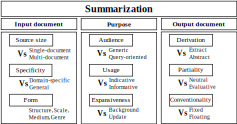
\includegraphics{figures/methods/sum-classif.pdf} % % %[width=140mm]
		\caption{Classification of summarization systems using different criteria.}
		\label{fig:summary-classif}
	\end{center}
\end{figure}

In this chapter, we will present each of these classifications in details with some examples. 
Each section will be reserved to one of the three classifications: input document, purpose and output document. 
Finally, we will discuss the impact of each method category on the multilingualism of the system (method).


\section{Input document focused summarization methods}

%======= Introduction ======= 
Examining the input document, a summarization system can be classified using three criteria: source size, specificity and form. 
Source size refers to how many documents a system can have as input. 
The specificity refers to the domains which this system can handle: is it designed just for a specific domain? or is it for general purpose? 
Input document(s) form specifies if they are structured or not, have low scale (tweets) or large one (novel), are textual or multimedia documents, and if they are of the same genre or not. 

%======= Source size ======= 
\subsection{Source size}

A summarization system can have one input document (single document) or many (multi-document) according to the source size criterion.
Some systems are designed to afford both single and multi-document summarization \citep{15-henss-al,15-aries-al}.
%definition
Single document systems process just one input document at once.
Even they use other documents for training, they still are using a single document as input. 
%works
This kind of summarization includes the first works of ATS \citep{58-luhn,58-baxendale,69-edmundson} as well as recent ones \citep{16-durrett-al,19-saini-al,19-liu-al}.
%benefit
It is simpler to process just one document since its sentences are more coherent and less redundant.
%limit
But, it is not adequate for all sort of applications.
For instance, if we want to summarize some news from different sources, we can end up with similar summaries if they talk about the same subject.

%definition
On the other hand, a multi-document system takes many documents of the same topic as input.
For example, summarizing news about a car crush from many newspapers. 
%works
The earliest work we can find in multi-document summarization is the work of \citet{95-mckeown-radev}. 
Some recent works focusing on this kind of summarization are \citep{15-zhong-al,19-tavir-al}.
%benefit 
The benefit of this type of summarization is to diversify information sources.
%limit
But, one of its most challenging issues is redundancy; documents talking about the same topic have much information in common.
%This classification (Single vs. Multi- document summarization) is very popular among researchers in the field of ATS. 


%======= Specificity ======= 
\subsection{Specificity}

An automatic summary can be generated from domain-specific documents or from general domains.
A domain is the general subject of a document; it can be high level such as sports, politics, science, etc. or low level such as football, tennis, etc. \citep{15-vander-al}.
%definition
Most works are not dedicated to a domain in particular even if they are tested on one. 
%works 
For instance, if someone uses cue words as in \citep{69-edmundson}, the method can be considered as domain-free (general) summarization. 
But, if these cue words are designed to favor some domain-related concepts such as medical domain \citep{09-sarkar}, in this case the method is domain specific. 
%benefits
In the end, general summarization systems can be beneficial since they can be applied to any domain. 
%limits
But, their performance will not be as good as domain-specific ones.


%definition
When we want to summarize documents of the same domain, it is more appropriate to use a summarization system specific to this domain. 
This can reduce terms ambiguities, the usage of grammar and formatting schemes. 
%works
Examples of domain-specific works: juridic texts \citep{04-farzindar-lapalme}, biomedical texts \citep{07-reeve-al}, medical texts \citep{09-sarkar,19-liang-al}.
%benefits
The performance of a domain-specific system should be better than a generic one, since it is designed for that matter.
%limits 
Designing such methods requires knowing the particularity of the domain so we can choose the right features.

%======= Form ======= 
\subsection{Form}

Input documents forms can be their structures, scales, mediums and genres. 
%definition
The structure refers to the explicit organization found in the document (eg. sections in papers: introduction, related works, method, experiments and conclusion).
The structure can be used to increase summarization performance where every section can be treated differently.
%works 
For instance, LetSumm system \citep{04-farzindar-lapalme} uses thematic structures in legal judgments (decision data, Introduction, Context, juridical analysis and Conclusion) to generate summaries. 
%For each thematic, some linguistic markers are affected to be used as cue phrases \citep{81-paice}. 
%The resulted summary is a combination of those thematic summaries with a percentage of contribution.
Another example is the work of \citet{07-pembe-gungor} who try to summarize \ac{html} documents. 
The sections are detected from \ac{html} tags to help reordering generated sentence
%benfits
Introducing document's structure helps summarization especially when users are more interested in a section than others. 
%limits
But, such methods can be applied to just the structures they are meant to work on.

%definition
The scale is another aspect which can affect the summarizing method; An input document can be a paragraph, an article, a book, etc. 
Many known summarization systems use term frequency as relevancy measure, therefore the input document must be large (important terms are repeated a lot).
%works
In case of summarizing low scale documents such as tweets \citet{10-sharifi-al,12-duan-al}, we cannot use usual techniques.
After all, a tweet is just as long as a summary itself. 
So, the summary is usually constructed from many tweets as input.
Some works limit the size of input document due to technical restrictions, such as using recurrent neural networks for abstractive summarization \citep{15-rush-al}. 
%benefits
Inventing new methods for different scales is a must when our documents have predefined sizes which can be as small as tweets or as large as encyclopedias.  
%limits 
These methods can face some challenges based on their specific scale.
If the document is too short, many known summarization techniques such as term frequency will not work on a single document.
If it is too large, processing time and memory can be an issue.

%definition
The medium is the support which carries the information.
Most summarization systems are based on textual support, while there are some researches on summarizing images, videos and audios.
%works
The work of \citet{14-gunhee-al} addresses the problem of jointly summarizing large-scale Flickr images and YouTube user videos. 
More works on multimedia summarization are: interactive football summarization \citep{09-moon}, summarizing important events in a football video \citep{12-zawbaa-al}, video summarization using web images \citep{13-khosla-al}, video summarization using a given category \citep{14-potapov-al}, video summarization by learning \citep{15-gygli-al,18-zho-al}.
%benefits 
Texts are not the only support that can benefit us when summarized; other supports such as multimedia content as abundant on the web as well.
%limits
These supports will not have the same methods as a text, and new methods must be adapted to each one.

%definition
Summarization systems can be classified using the genre of their input documents. 
A genre is defined as a complementary to domains covering non-topical text properties function, style,
and text type.  \citep{15-vander-al}.
As example, a document genres can be: news, interviews, reviews, novels, etc.
In this case, a method is created to support one genre, multiple genres or no genre at all (does not take genre in consideration).
%works
There are some works which adjust their scoring methods according to the document's genre.
The system is trained on multiple genres to select adequate features for each one \citep{07-goldstein-al} or to produce multiple summarization models for each genre \citep{10-yatsko-al}. 
Some systems are just designed for a specific genre, such as reviews \citep{09-zhan-al} and patents \citep{19-girthana-swamynathan}.
%benefits 
Specifying the genre of a method can be helpful especially when we are just interested in a very specific genre. 
%limits 
Though, it is not quit possible to defining a method for each genre. 


\section{Purpose focused summarization methods}

%======= Introduction ======= 
The purpose of summarization defines three criteria: audience, usage and expansiveness.
A summary audience specifies to whom it is intended: a specific user's profile or any user.  
The usage of summary can be helping users decide their interests or replacing the original document(s) as a shorter version of it.
As for the expansiveness, our definition is a little different from that of \citet{98-hovy-lin}. 
In our version, it is whether the summary have chronological knowledge of the past documents or not.

%======= Audience ======= 
\subsection{Audience}

Sometimes, users need a summary focusing on some aspects rather than the main idea of the input document. 
A summarization system which takes in consideration user's preferences is called query-oriented, while the one which does not is known as generic system. 
%definition
A generic summarization system tries to capture important information from an input document. 
So, we can say it tries to focus on the topic presented by the author and present what the input document is all about.
%works 
This type of systems exists widely, as an example: the systems in MultiLing'15 \citep{15-vanetik-litvak,15-aries-al,15-thomas-al,15-vicente-al}.
%benefits
This is beneficial if the readers are more interested in the main idea of a document.
%limits 
Nevertheless, sometimes readers are more interested in some subjects than others.

%definition
Query-oriented systems take in consideration users preferences.
For instance, if a user wants a summary focusing on someone in a story, it must contain events around this person without loosing the main interest of the story. 
%works
For instance, \citet{10-bhaskar-bandyopadhyay} describe a method to summarize multiple documents based on user queries.
The correlation measure between sentences from each document are calculated to create clusters of similar sentences.
Then, the sentences are scored according to the query.
This score is accumulated to the cluster score to extract the highest scored sentences.
Recent techniques such as deep learning have been used to generate query-oriented summaries \citep{15-zhong-al,19-kimuru-al}.
%benefilts
The benefit of query-oriented methods is clear: afford users with summaries based on their preferences.
%limits
The most challenging issue facing these methods is recovering query-relevant sentences of the documents that cover the main topics as well.

%======= Usage ======= 
\subsection{Usage}

A summary based on its usage is meant to help users decide their interests or as a representative replacement for the original document(s).
%definition
Informative summaries contain essential information of the original document(s); After reading them, you can tell what are the main ideas. 
This type of summaries can be found in journals, theses, research articles, etc. 
In a research article, the author must present the essential ideas and findings using an abstract which is considered as an informative summary.
%works
The majority of systems and methods focus on this type of summarization, hence we can find examples of this type anywhere.
%benefits
To sum up, Informative summaries are used as a short version of the input document(s).
%limits
Their main challenge is to express most ideas in the input document without redundancy.

Indicative summaries does not contain informative content; they only contain a global description of the original document. 
That includes the purpose, scope, and research methodology. 
This can be helpful to decide whether or not to consult the original document. 
The abstracts on the title page's verso of books and reports are an example of indicative summaries. 
Works have been conducted to investigate such type of summaries.
\citet{01-kan-al} propose an indicative multi-document summarization system (CENTRIFUSER) based on the problem of content planning. 
Figure \ref{fig:kan-al-exp} represents an example of a CENTRIFUSER summary on the health-care topic of ``Angina" where the generated indicative summary is in the bottom half using the difference in topic distribution of documents to regroup them.
%
\begin{figure}[ht]
	\begin{center}
		\includegraphics{figures/methods/kan-al-exp.pdf} % % %[width=140mm]
		\caption{An example of CENTRIFUSER summarizer output \citep{01-kan-al}.}
		\label{fig:kan-al-exp}
	\end{center}
\end{figure}
The method uses an IR system to search in a collection of documents, which gives a selected set of documents. 
Then some features are extracted from the collection and from the individual chosen documents to be used along with the query to generate the indicative summary.
%benefits
To sum up, Indicative summaries are used as a description to helping users select documents. 
%limits
Sometimes, it is more difficult to describe a document than finding out what it talks about. 
For instance, providing information about places (Where), persons (Who), etc. in a document.

%======= Expansiveness ======= 
\subsection{Expansiveness}

A generated summary can focus on original document's background, or afford the news compared to some past documents.
This property is referred to as expansiveness. 
A background summary, according to \citet{01-mani}, assumes that the reader has poor prior knowledge of general setting of the input text(s), and hence includes explanatory material, such as circumstances of place, time, and actors.
On the other hand, just-the-news summary is containing just novel or principal themes, assuming that the reader
knows enough background to interpret them in context. 
Nowadays, a lot of systems tend to afford the most relevant information found in input texts without verifying if the resulted summary incorporates some explanatory materials. 
Following the previous two definitions, these systems are neither background nor just-the-news. 
That is, such system can generate both background summaries and just-the-news ones. 
So, classifying systems based on whether or not they are designed to incorporate news is more appropriate.

%definition
Lets, first, redefine what just-the-news summaries and call them ``update summaries", since this term is more used. 
Recently, the emerging interest in systems that automatically monitor streams of social media posts such as Twitter or news to keep users up to date on topics they care about, led to the appearance of update summaries.
The idea is to generate summaries from some recent documents which do not contain information from previous documents. 
It means, the system must have prior knowledge of what has been seen before. 
%works
Update summaries were promoted in TAC 2008 as ``update task" \citep{08-dang-owczarzak} where the participants must generate multi-document update summaries from some chronologically ordered sets of news documents.
A more recent evaluation campaign for update summaries is ``Real-time summarization" task \citep{17-lin-al}.
%benefit
This type of summarization helps users to save time by reading just the news without consulting what they already know. 
%limits 
Besides the general challenges, update summarization must detect new information based on past documents. 
So, it has to take temporal information in consideration. 

%definition
We can, then, define a background summarization system as a system which generates summaries based on the input document(s) content and without excluding information from prior documents on the same subject. 
%works
Any system that does not have prior knowledge of past documents can be considered as a background summarization system. 
%benefits 
Compared to update summarization, this type can be used widely since it does not concern itself with documents chronological order.
%limits 
However, when this order is important to us, it is better to use update summarization over this one.

\section{Output document focused summarization methods}

Three criteria be used to classify a summarization system based on the summary: derivation, partiality and format.
Derivation means the fashion used to produce a summary from the original document, either by extracting relevant units or by creating a new text.
Partiality is how a summary handles the opinions found in the original document, which can be either neutral or evaluative.
As for format, the summary format can be fix or floating.

%===== Derivation ========
\subsection{Derivation}

It refers to the way used to obtain a summary. 
It can be by extracting pertinent units or by understanding and generating a new summary.
%definition
Extractive summaries are produced by, as the name says, extracting units from the original documents. 
Usually, these units are sentences because it is easy to keep the correctness of the summary's grammar.
%works
The first works in the field of \ac{ats} are extractive; they use some features to estimate the pertinence of a sentence.
Some of these features are: term frequency \citep{58-luhn}, position in the text \citep{58-baxendale,69-edmundson} and keywords \citep{69-edmundson}. 
Nowadays, this type of summarization is still widely applied \citep{17-ren-al,18-aries-al,19-liang-al}.
%benefits
What makes extractive methods so famous is their simplicity compared to the abstractive ones. 
They are simple to design, consuming less resources and giving good results.
%limits
However, they face many challenges such as informativeness and readability.

%information
Abstraction, on the other hand, is the generation of new text based on the input document(s).
Abstractive systems are difficult to design due to their heavy dependence on linguistic techniques.
Specifying the domain of a system can simplify the creation of this type of systems \citep{93-mitkov}.
%works 
The abstractive summary can be generated using a semantic representation of the text \citep{15-liu-al,19-barros-al,19-li-zhuge}.
Recently, many works try to generate abstractive summaries using deep learning \citep{15-rush-al,16-nallapati-al,17-ling-rush,19-you-al,19-shen-al}.
%benefits
Abstractive summaries are very important since they are similar to human abstracts. 
%limits
However, generating such summaries needs more resources in term of data, tools and processing time.

%===== Partiality ========
\subsection{Partiality}

Partiality, by definition, is the bias in favor of one thing over another. 
Following partiality criteria, a summarization system can be neutral or evaluative.
%Partiality~Neutral definition
A neutral system produces summaries which reflect the content of the input document(s) without judgment or evaluation. 
They are not designed to, specifically, include opinion into the summary even if the input document contains judgments.
%works
Most works fall into this class \citep{58-luhn,58-baxendale,69-edmundson,15-vanetik-litvak,15-aries-al,15-vicente-al,15-thomas-al,15-zhong-al}.
%benefits
The benefit of this type of methods is to present the general ideas in a document without trying to focus on opinions or giving some evaluations.
%limits
But, sometimes, some domains such as the juridical one needs more focus on evaluations than the main topic.

%Partiality~Evaluative definition
An evaluative system includes automatic judgments either implicitly or explicitly.
An explicit judgment can be seen as some statements of opinion included automatically.
The implicit one uses bias to include some material and omit another.
%works
A lot of examples can be afforded for this type of summarization, especially with the growth of interest towards users opinions. 
For instance, the work of \citet{16-othman-al} is based on summarizing customer opinions through Twitter. 
Given a conversation of tweets, the method tries to effectively extract the different product features as well as the polarity of the conversation messages.
The year 2008 knew the debut of a new task within TAC conference called ``Opinion Summarization task", which is meant to generate summaries from answers on opinion questions. 
%benefits
This kind of summarization can help us find opinions in reviews, legal judgments, etc.
It, also, allow us to generate summaries with some automatically generated opinions about a subject. 
%limits
Searching opinions in a document is not an easy task; it requires more knowledge of the type of documents. 

%======= Format ======
\subsection{Format}

Generated summaries must be presented using a format: as a list of sentences, as one paragraph, etc.
Some systems use a fixed format, while others present their summaries based on user preferences or based on some goals.
%definition 
A fixed format does not change from user to another or from summary purpose to another; it is always the same. 
%works
Most works fall into this class, since most of them are research systems which focus on the informational part of the summary rather than its format (presentation to the user).
%benefits 
Mostly, the generated summary is used to help users having a general idea about the documents; so, just one output format is enough.
%limits
However, with the variety of devices settings and users interests, this kind of summarization can be arguable.


%definition
Floating-situation summarization systems try to display the content of summaries using variable settings to a variety of readers for diverse purposes. 
%works
The ONTOSUM system \citep{05-bontcheva} is one of these systems; it uses device profile (e.g., mobile phone, Web browser) to adjust the summary formatting and length. 
Another similar work is given in \citep{18-chongtay-al} where the authors propose a responsive news summarization system for multiple mobile devices. 
%benefits 
This kind seeks to improving readability based on users settings and preferences.
%limits
To our knowledge, there are few works on floating situation summarization; all of them focus on responsive summary size.  


\section{Discussion}

% summarize the taxonomy
%========================
We presented different summarization categories based on the taxonomy found in \citep{98-hovy-lin,99-sparckjones}. 
%Our intention in this chapter is to present these methods and discuss their suitability for multilingual text summarization. 
%But before that, lets enlist the different categories. 
A method's categorization can be done based on three criteria: input document, purpose and output document. 
Looking to the input document, we can classify a method based on source size (multi-document, vs. mono-document), specificity (domain-specific vs. general) and form (structure, scale, medium and genre). 
The purpose of a summarization method contains three sub-criteria: audience (query-oriented vs. generic), usage (indicative vs. informative) and expansiveness (background vs. just-the-news).
We changed the definition of the last one (Expansiveness) to fit nowadays methods, this will categorize summaries into background or update.


% input document 
%=================
Lets start by assessing the impact of the input document categorization on multilingual text summarization. 
% source size
Source size has nothing to do with documents' languages. 
So, if a method is either multi-document or mono-document, this does not affect its multilingualism. 
Of course, if we want to go deep in processing multiple documents using their semantic relationships, in this case a multilingual method can be difficult to set in motion. 
% Specificity
Specificity criterion separates summarization methods into domain-specific and general. 
A domain-specific method uses language resources such as cue words to emphasize a domain over others, which makes it language-dependent. 
On the bright side, being dependent to a domain can help limiting the workload of adapting a certain system to a new language. 
For instance, it is fairly easy to prepare a list of domain words in a certain language, either manually or automatically. 
% form
Summarization systems based on document form are dependent to the structure, scale, medium and genre rather than the input language. 

% purpose
%==========
A summarization method can be categorized according to its purpose based on three criteria: audience, usage and expansiveness.
% Audience
According to the audience criterion a summary can be query-oriented or generic, both can be language independent.
In case of query-oriented methods, there is always a technique to consider users queries without relying on heavy language resources. 
For instance, cosine similarity can be used to calculate the pertinence of a sentence to the query based on their terms. 
% Usage
Looking to the summary's usage, a summary (and the method as well) can be indicative or informative.
An informative summary can be done without relying on heavy language resources. 
As for an indicative summary, if the purpose is to present a little text to invite the reader for reading the whole document, we can apply the  same analogy as informative one. 
If we want to present some information such as ``Who", ``When", ``Why", etc., in this case more language dependent resources are needed.
% Expansiveness
The expansiveness divides summaries into background and update summaries. 
Both of these categories can be generated without relying on heavy language resources.
For instance, in update summaries we can detect novelty using some statistical methods such as cosine similarity.

% Output document
%==========
A summarization method can be categorized according to its output document (the summary) based on three criteria: derivation, usage and expansiveness.
% Derivation
According to derivation, a summarization method can be extractive or abstractive.
The extractive one can rely only on statistical methods to extract some parts of the text, thus it can be language-independent. 
The abstractive, on the other hand, has to use some language information to generate new texts. 
Using Deep learning to produce new texts, the architecture itself is not designed for a specific language. 
But when it comes to the training set, we need a huge amount of text so the system learns a vocabulary and some generation rules. 
%This makes it so hard to adapt the system to many languages and 
% Partiality
According to partiality, a method (or a system) can be neutral or evaluative . 
The latter includes opinion, which can be implicit or explicit. 
Either ways, the system must rely on some language material to detect text opinions in case of implicit summarization, or to understand the text and generate opinions in case of explicit one. 
% Conventionality (Fixed, Floating)
The conventionality criterion, which divides methods into fixed or floating, has no relation with language. 


